\documentclass{article} % For LaTeX2e
\usepackage{nips14submit_e,times}
\usepackage{hyperref}
\usepackage{url}
\usepackage{amsthm,amsmath}
\usepackage{amssymb}
\usepackage{color}
\usepackage{algorithm}
\usepackage{graphicx}
%\documentstyle[nips14submit_09,times,art10]{article} % For LaTeX 2.09

\newtheorem{definition}{Definition}[section]
\newtheorem{theorem}{Theorem}[section]
\newtheorem{lemma}{Lemma}[section]
\newtheorem{corollary}{Corollary}[section]

\title{LISTA}

\author{
Anna Choromanska \\
Courant Institute of Mathematical Sciences \\
New York, NY, USA \\
\texttt{achoroma@cims.nyu.edu} \\
\And
Ross Goroshin \\
Courant Institute of Mathematical Sciences \\
New York, NY, USA \\
\texttt{goroshin@cims.nyu.edu} \\
\And
Pablo Sprechmann \\
Courant Institute of Mathematical Sciences \\
New York, NY, USA \\
\texttt{pablo@cims.nyu.edu} \\
\AND
Yann LeCun \\
Courant Institute of Mathematical Sciences, and Facebook\\
New York, NY, USA \\
\texttt{yann@cs.nyu.edu } 
}

% The \author macro works with any number of authors. There are two commands
% used to separate the names and addresses of multiple authors: \And and \AND.
%
% Using \And between authors leaves it to \LaTeX{} to determine where to break
% the lines. Using \AND forces a linebreak at that point. So, if \LaTeX{}
% puts 3 of 4 authors names on the first line, and the last on the second
% line, try using \AND instead of \And before the third author name.

\newcommand{\fix}{\marginpar{FIX}}
\newcommand{\new}{\marginpar{NEW}}

%\nipsfinalcopy % Uncomment for camera-ready version

\begin{document}

\maketitle

\begin{abstract}
\end{abstract}

\section{Motivation example for a single subspace}
In this section we illustrate on an example that there exists a space of yet not explored optimization tools which potentially might achieve faster convergence rate than standard optimizers by 'learning how to optimize'. In this section we restrict our analysis to the data living on a single linear subspace and in the next section we will consider a data living on the union of linear subspaces.

We are interested in the following optimization problem
\begin{eqnarray}
&&\min_{z_1,z_2,\dots,z_N} f(z_1,z_2,\dots,z_N),\text{\:\:\:where\:\:\:} \nonumber\\
&&f(z_1,z_2,\dots,z_N) = \sum_{i=1}^Nf(z_i) = \sum_{i=1}^N\|x_i - Wz_i\|^2 + \|z_i\|_1,
\label{eq:origin}
\end{eqnarray}
where $\mathcal{X} = \{x_1,x_2,\dots,x_N\}$ is the input dataset of cardinality $N$ and we assume data are independent identically distributed and have dimensionality $m$. The independence of the data points implies that each problem in Equation~\ref{eq:origin} can be solved separately. Furthermore, $W$ denotes the $m\times n$ dictionary matrix. 

As mentioned before we assume the data lives in a linear subspace. Therefore let $P$ be a $n \times n$ diagonal projection matrix with only $1$s and $0$s on a diagonal such that every data point lives in the range of matrix $WP$ thus for all $i = \{1,2,\dots,N\}$ there exists a real vector $\bar{z}_i \in \mathbb{R}^n$ such that
\[x_i = WP\bar{z}_i.
\]

Let $(z^{*}_1,z^{*}_2,\dots,z^{*}_N)$ denote the optimal solution of Equation~\ref{eq:origin}. Let $\{\Phi_1,\Phi_2,\dots,\Phi_N\}$ be a set of $n \times n$ diagonal projection matrices which are allowed to have $1$s only in these entrances where $P$ has $0$s (thus $P$ and $\Phi$ are orthogonal), and furthermore
\[z^{*}_i = (P + \Phi_i)z^{*}_i
\]
and $z^{*}_i \neq \Phi_i z^{*}_i$ thus $z^{*}_i$ does not belong to the nullspace of matrix $\Phi_i$.

We denote by $\epsilon$ the upper-bound on the following expression
\begin{equation}
\frac{1}{N}\sum_{i=1}^N(\bar{z}_i - z^{*}_i)^{\top}P^{\top}W^{\top}W\Phi_i z^{*}_i].
\label{eq:condition}
\end{equation}
This expression is in fact $\mathbb{E}[(\bar{z} - z^{*})^{\top}P^{\top}W^{\top}W\Phi z^{*}]$ and can be re-written as
\[\mathbb{E}[(\bar{z} - z^{*})^{\top}P^{\top}W^{\top}W\Phi z^{*}] = \mathbb{E}[(\bar{z} - z^{*})^{\top}P^{\top}W^{\top}W\Phi z^{*}] = \mathbb{E}[(x - WPz^{*})^{\top}W\Phi z^{*}].
\]
This expression will play a key role in our analysis. Note that $(x - WPz^{*})$ can be thought of as a measure of the reconstruction quality for data point $x\in\mathcal{X}$. It is in other words a vector $(\bar{z} - z^{*})$ projected on to the space where the data lives. On the other hand, $W\Phi z^{*}$ is a reconstruction residue. Thus $\epsilon$ is a measure of the average correlation between these two vectors. 

We will next show an interesting lemma motivating the idea of 'learning how to optimize'. 
\begin{theorem}
Let the following optimality condition hold
\[\epsilon \leq \frac{1}{N}\sum_{i=1}^N\|\Phi_i z^{*}_i\|_1 + \|W\Phi_i z^{*}_i\|^2.
\]
Then ISTA run on the following problem
\begin{eqnarray}
&&\min_{z_1,z_2,\dots,z_N} \tilde{f}(z_1,z_2,\dots,z_N), \text{\:\:\:where\:\:\:} \nonumber\\
&&\tilde{f}(z_1,z_2,\dots,z_N) = \sum_{i=1}^N\tilde{f}_i(z_i) = \sum_{i=1}^N\|x_i - WPz_i\|^2 + \|z_i\|_1,
\label{eq:modified}
\end{eqnarray}
recovers the optimal solution $(z^{*}_1,z^{*}_2,\dots,z^{*}_N)$ of the problem in Equation~\ref{eq:origin} and furthermore it does it faster than ISTA run directly on the problem in Equation~\ref{eq:origin}. Let $z_{i,k}$ be the sequence generated by ISTA run on the $i^{th}$ problem in Equation~\ref{eq:modified} (defined by the $i^{th}$ summand). Then for $k \geq 1$ the following holds
\begin{equation}
f(z_{1,k},z_{2,k},\dots,z_{N,k}) - f(z^{*}_1,z^{*}_2,\dots,z^{*}_N) \leq \sum_{i=1}^N\frac{\alpha\tilde{L}\|z_0 - z^{*}_i\|^2}{2k} \leq \sum_{i=1}^N\frac{\alpha L\|z_0 - z^{*}_i\|^2}{2k},
\label{eq:convrate}
\end{equation}
where $\tilde{L}$ (resp. $L$) is a Lipschitz constant of the gradient of $\tilde{s}(z) = \|x - WPz\|^2$ (resp. $s(z) = \|x - Wz\|^2)$ and $\alpha$ is the step size.
\label{thm:singlesubspace_simple}
\end{theorem}
Before proving the theorem, we a useful lemma that we will use later.
\begin{lemma}
Running ISTA on the each of the $i^{th}$ sub-problem in Equation~\ref{eq:modified} results in a sequence $\{z_{i,0},z_{i,1},\dots\}$ such that for all $k \in \{\mathbb{Z}\cup 0\}$ the following holds
\[Pz_{i,k} = z_{i,k}.
\]
\label{lem:Pzeqz}
\end{lemma}
\begin{proof}
Let $z_{i,0} = z_0 = 0$. Note that $z_{i,1} = h_{\theta_i}\left(\frac{1}{\tilde{L}}P^{\top}W^{\top}x_i\right) = Ph_{\theta_i}\left(\frac{1}{\tilde{L}}P^{\top}W^{\top}x_i\right)$, where the last equality is a consequence of the construction of matrix $P$. $h_{\theta_i}$ denotes the thresholding operation used by ISTA By the construction of matrix $P$ and from the induction assumption that $Pz_{i,k} = z_{i,k}$ it also follows that
$Pz_{i,k+1} = Ph_{\theta_i}\left(\frac{1}{\tilde{L}}P^{\top}W^{\top}x_i + \left(I - \frac{1}{\tilde{L}}P^{\top}W^{\top}WP\right)z_{i,k}\right) = h_{\theta_i}\left(\frac{1}{\tilde{L}}P^{\top}W^{\top}x_i + \left(I - \frac{1}{\tilde{L}}P^{\top}W^{\top}WP\right)z_{i,k}\right)$.
Thus by induction the lemma must hold.
\end{proof}

Lemma~\ref{lem:Pzeqz} implies that when running ISTA on the $i^{th}$ sub-problem in Equation~\ref{eq:modified} we get a sequence $\{z_{i,0},z_{0,1},\dots\}$ such that for any $k \in \{\mathbb{Z}\cup 0\}$ the following holds
\[\tilde{f}_i(z_{i,k}) = \|x_i - WPz_{i,k}\|^2 + \|z_{i,k}\|_1 = \|x_i - Wz_{i,k}\|^2 + \|z_{i,k}\|_1 = f_i(z_{i,k}).
\]
We will now prove Theorem~\ref{thm:singlesubspace_simple}.
\begin{proof}[Proof of Theorem~\ref{thm:singlesubspace_simple}]
Let $\tilde{z}^{*}$ be the optimal solution of problem in Equation~\ref{eq:modified}. Then by the guarantees of ISTA we have that
\[\tilde{f}(z_{1,k},z_{2,k},\dots,z_{N,k}) - \tilde{f}(\tilde{z}^{*}_1,\tilde{z}^{*}_2,\dots,\tilde{z}^{*}_N) \leq \sum_{i=1}^{N}\frac{\alpha\tilde{L}\|z_0 - \tilde{z}^{*}_i\|^2}{2k},
\]
and thus
\[f(z_{1,k},z_{2,k},\dots,z_{N,k}) - \tilde{f}(\tilde{z}^{*}_1,\tilde{z}^{*}_2,\dots,\tilde{z}^{*}_N) \leq \sum_{i=1}^{N}\frac{\alpha\tilde{L}\|z_0 - \tilde{z}^{*}_i\|^2}{2k}.
\]
Furthermore, note that 
\[\tilde{L} = 2\lambda_{\max}(P^{\top}W^{\top}WP) \leq 2\lambda_{\max}(W^{\top}W) = L
\]
thus 
\[f(z_{1,k},z_{2,k},\dots,z_{N,k}) - \tilde{f}(\tilde{z}^{*}_1,\tilde{z}^{*}_2,\dots,\tilde{z}^{*}_N) \leq \sum_{i=1}^{N}\frac{\alpha L\|z_0 - \tilde{z}^{*}_i\|^2}{2k}.
\]

Note that each $\tilde{z}^{*}_i$ lives in the range of matrix $P$. We will then show through contradiction that if the optimality condition holds then each $z^{*}_i$ also has to live in the range of $P$ (thus $\Phi_1 = \Phi_2 = \dots = \Phi_N = 0$). Suppose it is not true and recall $z^{*}_i = (P + \Phi_i)z^{*}_i$. Therefore
\begin{eqnarray*}
f(z^{*}_1,z^{*}_2,\dots,z^{*}_N) &=& \sum_{i=1}^N\|x_i - Wz^{*}_i\|^2  + \|z^{*}_i\|_1\\
&=& \sum_{i=1}^N\|x_i - W(P + \Phi_i)z^{*}_i\|^2 + \|(P + \Phi_i)z^{*}_i\|_1\\
&=& \sum_{i=1}^N\|x_i - WPz^{*}_i - W\Phi_i z^{*}_i\|^2 + \|Pz^{*}_i\|_1 + \|\Phi_i z^{*}_i\|_1,
\end{eqnarray*}
where the last equation comes from orthogonality of $Pz^{*}_i$ and $\Phi_i z^{*}_i$. We can further write that
\begin{eqnarray*}
f(z^{*}_1,z^{*}_2,\dots,z^{*}_N) &=& \sum_{i=1}^N\|WP\bar{z}_i - WPz^{*}_i - W\Phi_i z^{*}_i\|^2 + \|Pz^{*}_i\|_1 + \|\Phi_i z^{*}_i\|_1\\
&=& \sum_{i=1}^N\|WP(\bar{z}_i - z^{*}_i) - W\Phi_i z^{*}_i\|^2 + \|Pz^{*}_i\|_1 + \|\Phi_i z^{*}_i\|_1\\
&\geq& \sum_{i=1}^N\|WP(\bar{z}_i - z^{*}_i)\|^2 + \|W\Phi_i z^{*}_i\|^2 - \epsilon + \|Pz^{*}_i\|_1 + \|\Phi_i z^{*}_i\|_1\\
&=& f(Pz^{*}_1,Pz^{*}_2,\dots,Pz^{*}_N) + \sum_{i=1}^N\|\Phi_i z^{*}_i\|_1 + \|W\Phi_i z^{*}_i\|^2 - \epsilon\\
&\geq& f(Pz^{*}_1,Pz^{*}_2,\dots,Pz^{*}_N),
\end{eqnarray*}
where the last inequality results from the optimality condition.
\end{proof}

\newpage

\section{FLISTA}

\subsection{ISTA}

\begin{algorithm}
\caption{ISTA}
\begin{tabular}{l}
$Z = 0$\\
Repeat until change in $Z$ is below a threhold\\
\:\:\:\:\:$Z = Z - \frac{1}{L}W^{\top}(WZ-x)$ \:\:\:\:\:\:\:\:\:\:\:\:\:\:- gradient step\\
\:\:\:\:\:$Z = h_{\alpha/L}(Z)$ \:\:\:\:\:\:\:\:\:\:\:\:\:\:\:\:\:\:\:\:\:\:\:\:\:\:\:\:\:\:\:\:\:\:\:\:\:\:- thresholding step
\end{tabular}
\label{alg:ISTA}
\end{algorithm}

\begin{figure}[h]
  \center
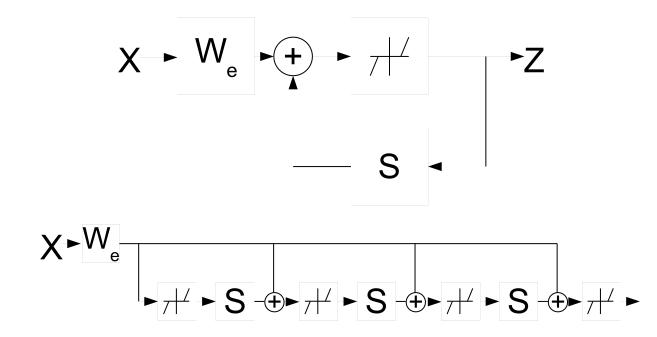
\includegraphics[width = 5in]{ISTAvsLISTA.jpg}
\caption{ISTA versus LISTA.}
\label{fig:ISTAvsLISTA}
\end{figure} 

\begin{algorithm}
\caption{FISTA}
\begin{tabular}{l}
Let $\lambda_0 = 0$, $\lambda_s = \frac{1 + \sqrt{1+4\lambda_{s-1}^2}}{2}$, and $\gamma_s = \frac{1-\lambda_s}{\lambda_{s+1}}$\\
$Z_0 = 0$\\
Repeat until change in $Z$ is below a threhold\\
\:\:\:\:\:$Z_{t+1} = Z_t - \frac{1}{L}W^{\top}(WZ_t-x)$ \:\:\:\:\:\:\:\:\:\:\:\:\:\:- gradient step\\
\:\:\:\:\:$Z_{t+1} = h_{\alpha/L}(Z_{t+1})$ \:\:\:\:\:\:\:\:\:\:\:\:\:\:\:\:\:\:\:\:\:\:\:\:\:\:\:\:\:\:\:\:\:\:\:- thresholding step\\
\:\:\:\:\:$Z_{t+1} = (1-\gamma_t)Z_{t+1} + \gamma_tZ_t$ \:\:\:\:\:\:\:\:\:\:\:\:\:\:\:\:\:\:\:- momentum step
\end{tabular}
\label{alg:FISTA}
\end{algorithm}



%\subsubsection*{Acknowledgments}

\small{
\bibliography{PAPER_ARPY}
\bibliographystyle{unsrt}
}

\end{document}
